\chapter{Application development}
\lhead{Chapter 3 \emph{Application development}}
\label{chap:3}
%\autoref{chap:3}
\bigskip

The mitigation of the overpopulation problem is nowadays an absolute necessity. The application, which is described below, has been developed towards this direction. More specifically, it can give the incentives to create space traffic management rules based on the orbit and capacity allocation, as well as the added value that each new satellite has.

The application has two major capabilities. The first one is the calculation of the revisit time of a single satellite or constellation (Section \ref{revisit time}). The second one is a tool, with which the user can find out what is the added value of an object based on the number of the satellites that are already in-orbit and have the same characteristics (Section \ref{added value}). This tool, in essence, has many more capabilities, which are presented in Chapter \ref{chap:4}.

\bigskip
\section{From satellite definition to revisit time calculation}
\label{revisit time}
\bigskip

The implementation of this first part of the application was programmed and carried out in Python. In this stage, the user defines a satellite by providing its two-line elements (TLE). However, since the application is focused only on the Earth Observation satellites, parameters related to this field are also necessary to be given.
%Write epigrammatika all the different steps here.

\bigskip
\subsection{Necessary input data}
\bigskip

In this first step, the user can define a satellite by providing the TLE set to the application. Despite the fact that the classical orbital elements are used in the scientific community, it was decided that the TLE set is a more convenient and fast way of importing and handling the input data, since the latter way is applied universally and the orbit computation in the next step can be done without any further conversions of those given parameters.

From the elements of a TLE set, eight parameters are being extracted and used in the application. Those are the epoch date, inclination ($i$), Right Ascension of the Ascending Node (RAAN) ($\Omega$), eccentricity ($e$), argument of perigee ($\omega$), mean anomaly ($M$), mean motion ($n$) and the international designator, which is a unique code of a satellite. In the Figure \ref{tle}, it can be seen an example dataset with all the information that TLE carries.

More specifically, the epoch date is the number of days passed in the particular year. The information about the year is taken from the first two digits of the parameter and from the following digits the exact month, day, epoch hour, minute and second can be found. Finally, the epoch time is calculated in seconds as:

\begin{equation}
epoch = (hour * 3600) + (min * 60) + sec.
\end{equation}

\begin{figure}
\centering
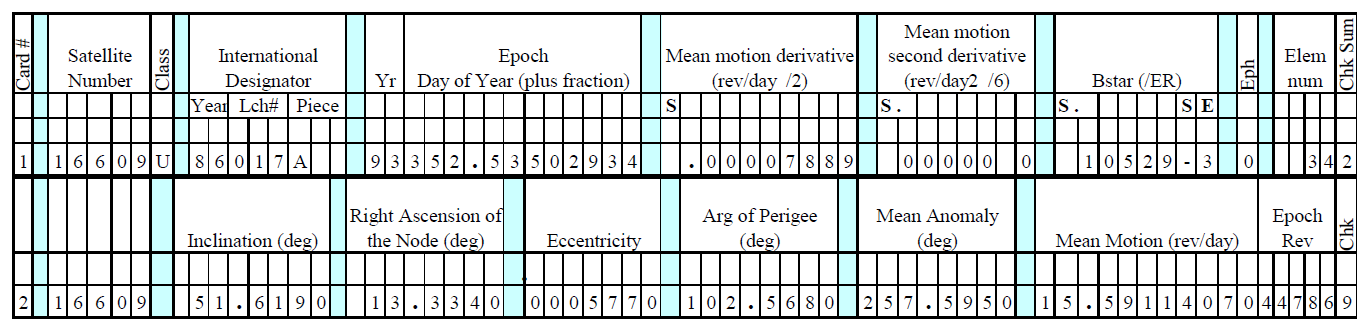
\includegraphics[width=0.9\textwidth]{Images/tle.png}\caption{An example two-line element (TLE) set. S is the sign of values, and E is of exponent. \textit{Source: \cite{Vallado}}}
\label{tle} 
\end{figure}

The parameters of eccentricity, inclination, RAAN, argument of perigee and mean anomaly can be seen graphically in the Figure \ref{keplerian_elements}. In short, eccentricity is a constant defining the shape of the orbit. There is a circular orbit when it is zero and an elliptical orbit when the number is less than one. To the given value of eccentricity from the TLE, a decimal at the beginning must be applied. As far as the inclination, which is given in degrees, it is the angle between the equator and the orbit plane. The RAAN (degrees) is the angle between vernal equinox and the point where the orbit crosses the equatorial plane and goes towards the north. Argument of perigee, or else the node is the angle between the ascending node and the orbit's point of the closest approach to the earth, which is called perigee. It is given in degrees. Finally, the mean anomaly is the angle of satellite location in the nominal orbit, which referenced to a circular orbit with radius equal to the semi-major axis. It is measured from the perigee and it is also given in degrees. It should be also noted that the conversion of their units from degrees to radians is necessary, since many other computations will be followed. \cite{Vallado}

From the parameter of mean motion ($n$), the semi-major axis ($a$), as well as the period ($T$) of the orbit can be found. Namely, the mean motion is converted from the unit of $revolutions/day$ to $radian/sec$. Then, the semi-major axis is calculated from the Kepler's 3\textsuperscript{nd} law:
\begin{equation}
n^2 * a^3 = \mu,
\end{equation}
%a = (\frac{\mu}{n^2})^{1/3},
with $\mu$ being the geometric gravitational parameter.

\begin{figure}
\centering
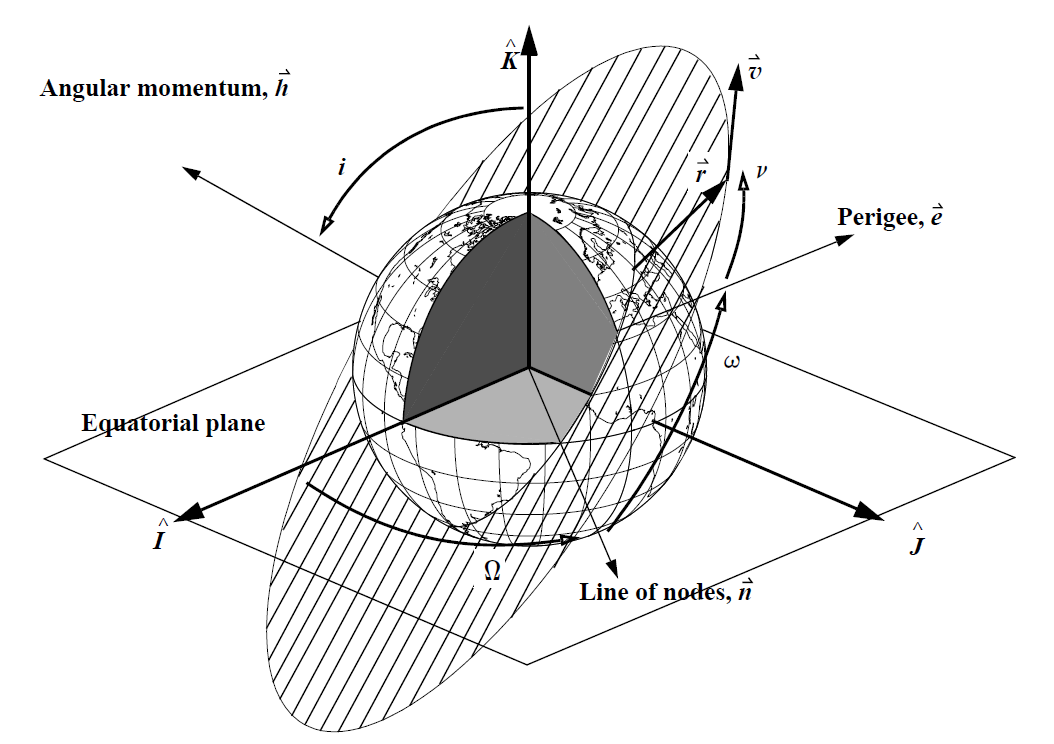
\includegraphics[width=0.9\textwidth]{Images/keplerian_elements.png}\caption{The classical orbital elements: semi-major axis ($a$), eccentricty ($e$), inclination ($i$), Right Ascension of the Ascending Node (RAAN) ($\Omega$), argument of perigee ($\omega$), and true anomaly ($\nu$). \textit{Source: \cite{Vallado}}}
\label{keplerian_elements} 
\end{figure}

Apart from the parameters that were just mentioned, it is necessary to be added some parameters related to the Earth Observation sensor that the satellite has. The orbit lifetime, the type of sensor (see Section \ref{EO}) and the resolution are some of them. However, the determiner parameter in the calculation of the revisit time is the information of the swath width of the sensor, which is further explained in the following section. The number is inserted in the units of kilometers.

\bigskip
\subsection{Orbit computation}
\bigskip


%Conversion to the correct units
%Semester 1 - Ex1 + Tutorial

%Book: Montenbruck


\bigskip
\subsubsection{Revisit time definition}
\bigskip

% Define revisit time --> average (median) revisit time in equator
%ABOUT REVISIT TIME:
%The interval of time required for the satellite to complete its orbit cycle is not the same as the "revisit period". Due to the steerable sensors, the off-nadir angles, the large swath width , the revisit time can be less than the orbit cycle time. "The revisit period is an important consideration for a number of monitoring applications, especially when frequent imaging is required (for example, to monitor the spread of an oil spill, or the extent of flooding). In near-polar orbits, areas at high latitudes will be imaged more frequently than the equatorial zone due to the increasing overlap in adjacent swaths as the orbit paths come closer together near the poles." (Source: https://www.nrcan.gc.ca/maps-tools-and-publications/satellite-imagery-and-air-photos/remote-sensing-tutorials/acknowledgements-permission-use/9391)

\subsection{Computational calculation of revisit time}

In order to approach the issue of calculating the revisit time in equator The swath width of the sensor (?) defines somehow the "area". 

\subsubsection{Map projection}

%Print earth map. Based on the FOV and the revisit frequency, I can see how the Earth will be printed/colored (heat map). So, we want to track coverage/ revisit time across the equator.

% Tip: "Do not present data at this stage but use sketches or synthetic data instead"






%(If I want to further analyze about the satellite viewing geometries and scanning patterns: Page 21,22 in http://www.atmosp.physics.utoronto.ca/people/strong/phy499/section2_05.pdf) --> It makes sense to do it if a use different ways to calculate the revisit time. So, if for every satellite I have the detailed info about the viewing geometry then I can do it. Another way is to write those info in the theory part and then calculate the revisit time, since I don't have much info ...

%As far as the Space-Time Sampling in the LEO satellites: a) sampling is highly dependent on the orbit, b) area viewed on one orbit overlaps area viewed on the previous and succeeding orbits, c) usually view every point on the Earth twice a day, d) view each point a small number of local times but at varying elevation and azimuth angles.

\bigskip
\section{Added value of satellite based on operational similar objects}
\label{added value}
\bigskip

\bigskip
\subsection{Database}
\bigskip
% Mention the focus on LEO and EO satellites
% Implemented in PostgreSQL

%In the chapter, where you will talk about the database, add big tables about the results - with the commercial and non-commercial constellations & then put a reference next to the other table that I have only the commercial EO satellites in the "Chapter_1" (~ Seira 234)!

%\section{Sources of data}
%\bigskip
%
%\section{Data gathering procedure}
%\bigskip

\bigskip
\subsection{Classification of Earth Observation field}
\bigskip


% Different import ways of adding data


